% Options for packages loaded elsewhere
\PassOptionsToPackage{unicode}{hyperref}
\PassOptionsToPackage{hyphens}{url}
%
\documentclass[
]{book}
\usepackage{lmodern}
\usepackage{amssymb,amsmath}
\usepackage{ifxetex,ifluatex}
\ifnum 0\ifxetex 1\fi\ifluatex 1\fi=0 % if pdftex
  \usepackage[T1]{fontenc}
  \usepackage[utf8]{inputenc}
  \usepackage{textcomp} % provide euro and other symbols
\else % if luatex or xetex
  \usepackage{unicode-math}
  \defaultfontfeatures{Scale=MatchLowercase}
  \defaultfontfeatures[\rmfamily]{Ligatures=TeX,Scale=1}
\fi
% Use upquote if available, for straight quotes in verbatim environments
\IfFileExists{upquote.sty}{\usepackage{upquote}}{}
\IfFileExists{microtype.sty}{% use microtype if available
  \usepackage[]{microtype}
  \UseMicrotypeSet[protrusion]{basicmath} % disable protrusion for tt fonts
}{}
\makeatletter
\@ifundefined{KOMAClassName}{% if non-KOMA class
  \IfFileExists{parskip.sty}{%
    \usepackage{parskip}
  }{% else
    \setlength{\parindent}{0pt}
    \setlength{\parskip}{6pt plus 2pt minus 1pt}}
}{% if KOMA class
  \KOMAoptions{parskip=half}}
\makeatother
\usepackage{xcolor}
\IfFileExists{xurl.sty}{\usepackage{xurl}}{} % add URL line breaks if available
\IfFileExists{bookmark.sty}{\usepackage{bookmark}}{\usepackage{hyperref}}
\hypersetup{
  pdftitle={Indicateurs de la Biodiversité},
  pdfauthor={Andrew MacDonald},
  hidelinks,
  pdfcreator={LaTeX via pandoc}}
\urlstyle{same} % disable monospaced font for URLs
\usepackage{color}
\usepackage{fancyvrb}
\newcommand{\VerbBar}{|}
\newcommand{\VERB}{\Verb[commandchars=\\\{\}]}
\DefineVerbatimEnvironment{Highlighting}{Verbatim}{commandchars=\\\{\}}
% Add ',fontsize=\small' for more characters per line
\usepackage{framed}
\definecolor{shadecolor}{RGB}{248,248,248}
\newenvironment{Shaded}{\begin{snugshade}}{\end{snugshade}}
\newcommand{\AlertTok}[1]{\textcolor[rgb]{0.94,0.16,0.16}{#1}}
\newcommand{\AnnotationTok}[1]{\textcolor[rgb]{0.56,0.35,0.01}{\textbf{\textit{#1}}}}
\newcommand{\AttributeTok}[1]{\textcolor[rgb]{0.77,0.63,0.00}{#1}}
\newcommand{\BaseNTok}[1]{\textcolor[rgb]{0.00,0.00,0.81}{#1}}
\newcommand{\BuiltInTok}[1]{#1}
\newcommand{\CharTok}[1]{\textcolor[rgb]{0.31,0.60,0.02}{#1}}
\newcommand{\CommentTok}[1]{\textcolor[rgb]{0.56,0.35,0.01}{\textit{#1}}}
\newcommand{\CommentVarTok}[1]{\textcolor[rgb]{0.56,0.35,0.01}{\textbf{\textit{#1}}}}
\newcommand{\ConstantTok}[1]{\textcolor[rgb]{0.00,0.00,0.00}{#1}}
\newcommand{\ControlFlowTok}[1]{\textcolor[rgb]{0.13,0.29,0.53}{\textbf{#1}}}
\newcommand{\DataTypeTok}[1]{\textcolor[rgb]{0.13,0.29,0.53}{#1}}
\newcommand{\DecValTok}[1]{\textcolor[rgb]{0.00,0.00,0.81}{#1}}
\newcommand{\DocumentationTok}[1]{\textcolor[rgb]{0.56,0.35,0.01}{\textbf{\textit{#1}}}}
\newcommand{\ErrorTok}[1]{\textcolor[rgb]{0.64,0.00,0.00}{\textbf{#1}}}
\newcommand{\ExtensionTok}[1]{#1}
\newcommand{\FloatTok}[1]{\textcolor[rgb]{0.00,0.00,0.81}{#1}}
\newcommand{\FunctionTok}[1]{\textcolor[rgb]{0.00,0.00,0.00}{#1}}
\newcommand{\ImportTok}[1]{#1}
\newcommand{\InformationTok}[1]{\textcolor[rgb]{0.56,0.35,0.01}{\textbf{\textit{#1}}}}
\newcommand{\KeywordTok}[1]{\textcolor[rgb]{0.13,0.29,0.53}{\textbf{#1}}}
\newcommand{\NormalTok}[1]{#1}
\newcommand{\OperatorTok}[1]{\textcolor[rgb]{0.81,0.36,0.00}{\textbf{#1}}}
\newcommand{\OtherTok}[1]{\textcolor[rgb]{0.56,0.35,0.01}{#1}}
\newcommand{\PreprocessorTok}[1]{\textcolor[rgb]{0.56,0.35,0.01}{\textit{#1}}}
\newcommand{\RegionMarkerTok}[1]{#1}
\newcommand{\SpecialCharTok}[1]{\textcolor[rgb]{0.00,0.00,0.00}{#1}}
\newcommand{\SpecialStringTok}[1]{\textcolor[rgb]{0.31,0.60,0.02}{#1}}
\newcommand{\StringTok}[1]{\textcolor[rgb]{0.31,0.60,0.02}{#1}}
\newcommand{\VariableTok}[1]{\textcolor[rgb]{0.00,0.00,0.00}{#1}}
\newcommand{\VerbatimStringTok}[1]{\textcolor[rgb]{0.31,0.60,0.02}{#1}}
\newcommand{\WarningTok}[1]{\textcolor[rgb]{0.56,0.35,0.01}{\textbf{\textit{#1}}}}
\usepackage{longtable,booktabs}
% Correct order of tables after \paragraph or \subparagraph
\usepackage{etoolbox}
\makeatletter
\patchcmd\longtable{\par}{\if@noskipsec\mbox{}\fi\par}{}{}
\makeatother
% Allow footnotes in longtable head/foot
\IfFileExists{footnotehyper.sty}{\usepackage{footnotehyper}}{\usepackage{footnote}}
\makesavenoteenv{longtable}
\usepackage{graphicx}
\makeatletter
\def\maxwidth{\ifdim\Gin@nat@width>\linewidth\linewidth\else\Gin@nat@width\fi}
\def\maxheight{\ifdim\Gin@nat@height>\textheight\textheight\else\Gin@nat@height\fi}
\makeatother
% Scale images if necessary, so that they will not overflow the page
% margins by default, and it is still possible to overwrite the defaults
% using explicit options in \includegraphics[width, height, ...]{}
\setkeys{Gin}{width=\maxwidth,height=\maxheight,keepaspectratio}
% Set default figure placement to htbp
\makeatletter
\def\fps@figure{htbp}
\makeatother
\setlength{\emergencystretch}{3em} % prevent overfull lines
\providecommand{\tightlist}{%
  \setlength{\itemsep}{0pt}\setlength{\parskip}{0pt}}
\setcounter{secnumdepth}{5}
\usepackage{booktabs}
\usepackage[]{natbib}
\bibliographystyle{apalike}

\title{Indicateurs de la Biodiversité}
\author{Andrew MacDonald}
\date{2020-06-29}

\begin{document}
\maketitle

{
\setcounter{tocdepth}{1}
\tableofcontents
}
\hypertarget{dependencies}{%
\chapter{Dependencies}\label{dependencies}}

\begin{Shaded}
\begin{Highlighting}[]
\KeywordTok{library}\NormalTok{(rcoleo)}
\KeywordTok{library}\NormalTok{(tidyverse)}
\KeywordTok{library}\NormalTok{(lubridate)}
\end{Highlighting}
\end{Shaded}

\hypertarget{dl}{%
\chapter{Download data}\label{dl}}

The only point here is to demonstrate the workflow for downloading data

\begin{Shaded}
\begin{Highlighting}[]
\CommentTok{\# On retire les cellules (classe sf) depuis l\textquotesingle{}API}
\NormalTok{cells \textless{}{-}}\StringTok{ }\NormalTok{rcoleo}\OperatorTok{::}\KeywordTok{sf\_cells}\NormalTok{()}
\NormalTok{obs \textless{}{-}}\StringTok{ }\NormalTok{rcoleo}\OperatorTok{::}\KeywordTok{get\_obs}\NormalTok{()}
\NormalTok{sites\_dl \textless{}{-}}\StringTok{ }\NormalTok{rcoleo}\OperatorTok{::}\KeywordTok{sf\_sites}\NormalTok{()}

\CommentTok{\# until there is a better way to obtain the data and parse the result (perhaps}
\CommentTok{\# in the form of a convenience function in rcoleo) we do this:}

\NormalTok{obs\_df \textless{}{-}}\StringTok{ }\NormalTok{obs[[}\DecValTok{1}\NormalTok{]] }\OperatorTok{\%\textgreater{}\%}\StringTok{ }\KeywordTok{map}\NormalTok{(}\StringTok{"body"}\NormalTok{) }\OperatorTok{\%\textgreater{}\%}\StringTok{ }\KeywordTok{map\_df}\NormalTok{(}\OperatorTok{\textasciitilde{}}\StringTok{ }\KeywordTok{select}\NormalTok{(.x, }\OperatorTok{{-}}\NormalTok{closed\_at))}

\NormalTok{all\_obs \textless{}{-}}\StringTok{ }\NormalTok{obs\_df }\OperatorTok{\%\textgreater{}\%}
\StringTok{  }\KeywordTok{select}\NormalTok{(cell\_code, site\_code, date\_obs, type, }
         \DataTypeTok{taxa =}\NormalTok{ obs\_species.taxa\_name, }
         \DataTypeTok{var =}\NormalTok{ obs\_species.variable, }
         \DataTypeTok{val =}\NormalTok{ obs\_species.value) }\OperatorTok{\%\textgreater{}\%}\StringTok{ }
\StringTok{  }\KeywordTok{mutate}\NormalTok{(}\DataTypeTok{date\_obs =}\NormalTok{ lubridate}\OperatorTok{::}\KeywordTok{ymd}\NormalTok{(date\_obs),}
         \CommentTok{\# convert cover into pres/abs (right?)}
         \DataTypeTok{count =} \KeywordTok{if\_else}\NormalTok{(var }\OperatorTok{==}\StringTok{ "recouvrement"}\NormalTok{, }\DecValTok{1}\NormalTok{, val))}

\CommentTok{\# CELLULES: On compte le nombre d\textquotesingle{}observation/nombre espece par type, année et cellule}
\NormalTok{obs\_cells \textless{}{-}}\StringTok{ }\NormalTok{all\_obs }\OperatorTok{\%\textgreater{}\%}\StringTok{ }
\StringTok{  }\KeywordTok{group\_by}\NormalTok{(cell\_code, date\_obs, type) }\OperatorTok{\%\textgreater{}\%}\StringTok{ }
\StringTok{  }\KeywordTok{summarise}\NormalTok{(}\DataTypeTok{n =} \KeywordTok{sum}\NormalTok{(count)) }\OperatorTok{\%\textgreater{}\%}\StringTok{ }
\StringTok{  }\NormalTok{ungroup}

\NormalTok{sp\_cells \textless{}{-}}\StringTok{  }\NormalTok{all\_obs }\OperatorTok{\%\textgreater{}\%}\StringTok{ }
\StringTok{  }\KeywordTok{select}\NormalTok{(cell\_code, date\_obs, type, taxa) }\OperatorTok{\%\textgreater{}\%}\StringTok{ }
\StringTok{  }\KeywordTok{distinct}\NormalTok{() }\OperatorTok{\%\textgreater{}\%}\StringTok{ }
\StringTok{  }\KeywordTok{group\_by}\NormalTok{(cell\_code, date\_obs, type) }\OperatorTok{\%\textgreater{}\%}
\StringTok{  }\KeywordTok{summarise}\NormalTok{(}\DataTypeTok{n =} \KeywordTok{n}\NormalTok{()) }\OperatorTok{\%\textgreater{}\%}\StringTok{ }
\StringTok{  }\NormalTok{ungroup}

\CommentTok{\# CAMPAGNES}
\NormalTok{sites \textless{}{-}}\StringTok{ }\NormalTok{sites\_dl }\OperatorTok{\%\textgreater{}\%}\StringTok{ }
\StringTok{  }\KeywordTok{select}\NormalTok{(site\_code, off\_station\_code\_id,}
         \DataTypeTok{type\_milieu =}\NormalTok{ type, geometry, }\DataTypeTok{site\_id =}\NormalTok{ id)}

\CommentTok{\# On prépare les jeux de données pour chacun des types de campagnes}

\NormalTok{all\_obs\_con \textless{}{-}}\StringTok{  }\NormalTok{all\_obs }\OperatorTok{\%\textgreater{}\%}
\StringTok{  }\KeywordTok{filter}\NormalTok{(taxa }\OperatorTok{!=}\StringTok{ "inconnu"}\NormalTok{)}

\NormalTok{microfaunes \textless{}{-}}\StringTok{ }\KeywordTok{subset}\NormalTok{(all\_obs\_con, type }\OperatorTok{==}\StringTok{ "insectes\_sol"}\NormalTok{)}

\NormalTok{papillons \textless{}{-}}\StringTok{ }\KeywordTok{subset}\NormalTok{(all\_obs\_con, type }\OperatorTok{==}\StringTok{ "papilionidés"}\NormalTok{)}

\NormalTok{odonates \textless{}{-}}\StringTok{ }\KeywordTok{subset}\NormalTok{(all\_obs\_con, type }\OperatorTok{==}\StringTok{ "odonates"}\NormalTok{)}

\NormalTok{vegetation \textless{}{-}}\StringTok{ }\KeywordTok{subset}\NormalTok{(all\_obs\_con, type }\OperatorTok{==}\StringTok{ "végétation"}\NormalTok{)}
\end{Highlighting}
\end{Shaded}

\hypertarget{overall-summary}{%
\subsection{overall summary}\label{overall-summary}}

\begin{Shaded}
\begin{Highlighting}[]
\NormalTok{all\_obs\_con }\OperatorTok{\%\textgreater{}\%}\StringTok{ }
\StringTok{  }\KeywordTok{group\_by}\NormalTok{(type) }\OperatorTok{\%\textgreater{}\%}\StringTok{ }
\StringTok{  }\KeywordTok{summarize}\NormalTok{(}\DataTypeTok{sites =} \KeywordTok{n\_distinct}\NormalTok{(site\_code),}
            \DataTypeTok{cells =} \KeywordTok{n\_distinct}\NormalTok{(cell\_code),}
            \DataTypeTok{taxa =} \KeywordTok{n\_distinct}\NormalTok{(taxa))}
\end{Highlighting}
\end{Shaded}

\begin{verbatim}
## `summarise()` ungrouping output (override with `.groups` argument)
\end{verbatim}

\begin{verbatim}
## # A tibble: 4 x 4
##   type         sites cells  taxa
##   <chr>        <int> <int> <int>
## 1 insectes_sol    13    13    37
## 2 odonates        12    10    35
## 3 papilionidés    14    11    26
## 4 végétation      26    11   170
\end{verbatim}

\hypertarget{sites}{%
\chapter{Sites}\label{sites}}

Summary data about the different sites

\begin{Shaded}
\begin{Highlighting}[]
\NormalTok{obs\_cells }\OperatorTok{\%\textgreater{}\%}\StringTok{ }
\StringTok{  }\KeywordTok{ggplot}\NormalTok{(}\KeywordTok{aes}\NormalTok{(}\DataTypeTok{x =}\NormalTok{ cell\_code, }\DataTypeTok{y =}\NormalTok{ n)) }\OperatorTok{+}\StringTok{ }\KeywordTok{geom\_point}\NormalTok{() }\OperatorTok{+}\StringTok{ }
\StringTok{  }\KeywordTok{facet\_wrap}\NormalTok{(}\OperatorTok{\textasciitilde{}}\NormalTok{type, }\DataTypeTok{scales =} \StringTok{"free\_y"}\NormalTok{)}
\end{Highlighting}
\end{Shaded}

\begin{verbatim}
## Warning: Removed 1 rows containing missing values (geom_point).
\end{verbatim}

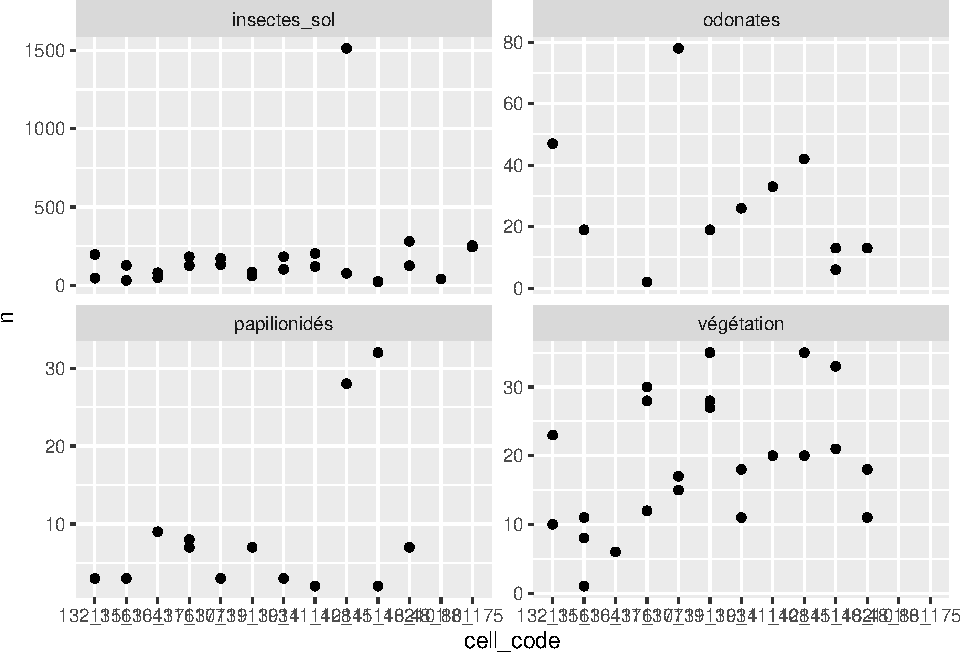
\includegraphics{indicators-bookdown_files/figure-latex/site_plot-1.pdf}

\hypertarget{odonate-communities}{%
\chapter{Odonate communities}\label{odonate-communities}}

\begin{Shaded}
\begin{Highlighting}[]
\CommentTok{\# confirm that the only variable recorded here is "abondance"}
\NormalTok{odonates}\OperatorTok{$}\NormalTok{var }\OperatorTok{\%\textgreater{}\%}\StringTok{ }\NormalTok{unique }\OperatorTok{\%\textgreater{}\%}\StringTok{ }\NormalTok{\{}\KeywordTok{stopifnot}\NormalTok{(. }\OperatorTok{==}\StringTok{ "abondance"}\NormalTok{)\}}

\NormalTok{odonates }\OperatorTok{\%\textgreater{}\%}\StringTok{ }
\StringTok{  }\NormalTok{glimpse }\OperatorTok{\%\textgreater{}\%}\StringTok{ }
\StringTok{  }\NormalTok{\{}\KeywordTok{all.equal}\NormalTok{(.}\OperatorTok{$}\NormalTok{count, .}\OperatorTok{$}\NormalTok{val)\}}
\end{Highlighting}
\end{Shaded}

\begin{verbatim}
## Rows: 151
## Columns: 8
## $ cell_code <chr> "135_104", "135_104", "135_104", "135_104", "135_104", "1...
## $ site_code <chr> "135_104_H01", "135_104_H01", "135_104_H01", "135_104_H01...
## $ date_obs  <date> 2016-06-23, 2016-06-23, 2016-06-23, 2016-06-23, 2016-06-...
## $ type      <chr> "odonates", "odonates", "odonates", "odonates", "odonates...
## $ taxa      <chr> "Leucorrhinia hudsonica", "Nehalennia gracilis", "Gomphus...
## $ var       <chr> "abondance", "abondance", "abondance", "abondance", "abon...
## $ val       <dbl> 2, 1, 1, 1, 1, 1, 1, 2, 1, 1, 2, 4, 1, 10, 1, 30, 5, 20, ...
## $ count     <dbl> 2, 1, 1, 1, 1, 1, 1, 2, 1, 1, 2, 4, 1, 10, 1, 30, 5, 20, ...
\end{verbatim}

\begin{verbatim}
## [1] TRUE
\end{verbatim}

\begin{Shaded}
\begin{Highlighting}[]
\CommentTok{\#\# are sites nested in cells? }

\NormalTok{odonates }\OperatorTok{\%\textgreater{}\%}\StringTok{ }
\StringTok{  }\KeywordTok{select}\NormalTok{(site\_code, cell\_code) }\OperatorTok{\%\textgreater{}\%}\StringTok{ }\NormalTok{distinct }\OperatorTok{\%\textgreater{}\%}\StringTok{ }
\StringTok{  }\KeywordTok{group\_by}\NormalTok{(cell\_code) }\OperatorTok{\%\textgreater{}\%}\StringTok{ }\NormalTok{tally}
\end{Highlighting}
\end{Shaded}

\begin{verbatim}
## # A tibble: 10 x 2
##    cell_code     n
##    <chr>     <int>
##  1 132_116       1
##  2 135_104       1
##  3 137_107       1
##  4 137_111       1
##  5 139_103       1
##  6 139_111       1
##  7 141_108       1
##  8 142_111       2
##  9 145_102       2
## 10 148_101       1
\end{verbatim}

\begin{Shaded}
\begin{Highlighting}[]
\CommentTok{\# yes, sometimes there are sites within cells!}
\end{Highlighting}
\end{Shaded}

\begin{Shaded}
\begin{Highlighting}[]
\NormalTok{rank\_abundance \textless{}{-}}\StringTok{ }\NormalTok{odonates }\OperatorTok{\%\textgreater{}\%}\StringTok{ }
\StringTok{  }\KeywordTok{left\_join}\NormalTok{(}\KeywordTok{select}\NormalTok{(cells, cell\_code, name)) }\OperatorTok{\%\textgreater{}\%}\StringTok{ }
\StringTok{  }\KeywordTok{group\_by}\NormalTok{(cell\_code, name, site\_code, taxa) }\OperatorTok{\%\textgreater{}\%}\StringTok{ }
\StringTok{  }\KeywordTok{summarize}\NormalTok{(}\DataTypeTok{total =} \KeywordTok{sum}\NormalTok{(count)) }\OperatorTok{\%\textgreater{}\%}\StringTok{ }
\StringTok{  }\KeywordTok{mutate}\NormalTok{(}\DataTypeTok{rank =} \KeywordTok{row\_number}\NormalTok{(}\KeywordTok{desc}\NormalTok{(total)))}
\end{Highlighting}
\end{Shaded}

\begin{verbatim}
## Joining, by = "cell_code"
\end{verbatim}

\begin{verbatim}
## `summarise()` regrouping output by 'cell_code', 'name', 'site_code' (override with `.groups` argument)
\end{verbatim}

\begin{Shaded}
\begin{Highlighting}[]
\NormalTok{rank\_abundance }\OperatorTok{\%\textgreater{}\%}\StringTok{ }
\StringTok{  }\KeywordTok{ggplot}\NormalTok{(}\KeywordTok{aes}\NormalTok{(}\DataTypeTok{x =}\NormalTok{ rank, }\DataTypeTok{y =}\NormalTok{ total, }\DataTypeTok{group =}\NormalTok{ site\_code)) }\OperatorTok{+}\StringTok{ }
\StringTok{  }\KeywordTok{geom\_point}\NormalTok{() }\OperatorTok{+}\StringTok{ }
\StringTok{  }\KeywordTok{geom\_line}\NormalTok{() }\OperatorTok{+}\StringTok{ }
\StringTok{  }\KeywordTok{facet\_wrap}\NormalTok{(}\OperatorTok{\textasciitilde{}}\NormalTok{name) }\OperatorTok{+}\StringTok{ }
\StringTok{  }\KeywordTok{coord\_trans}\NormalTok{(}\DataTypeTok{y =} \StringTok{"log"}\NormalTok{) }\OperatorTok{+}\StringTok{ }
\StringTok{  }\KeywordTok{theme\_bw}\NormalTok{()}
\end{Highlighting}
\end{Shaded}

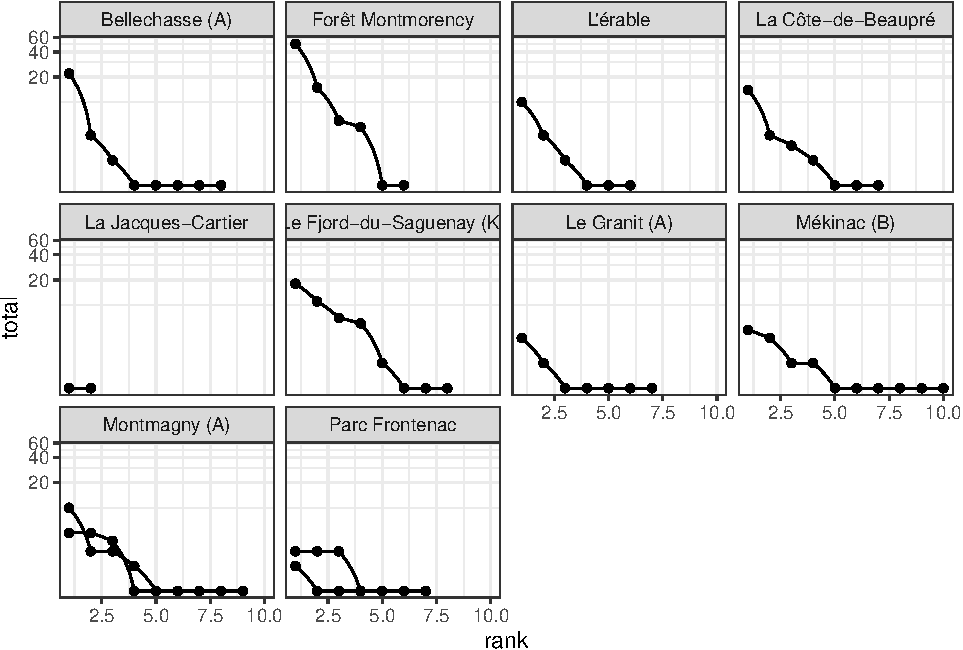
\includegraphics{indicators-bookdown_files/figure-latex/fig_rank_abd_odonate-1.pdf}

\hypertarget{questions}{%
\section{Questions}\label{questions}}

Some sites appear to count \textbf{individuals}, not species? why is that?

\begin{Shaded}
\begin{Highlighting}[]
\NormalTok{odonates }\OperatorTok{\%\textgreater{}\%}\StringTok{ }
\StringTok{  }\KeywordTok{left\_join}\NormalTok{(}\KeywordTok{select}\NormalTok{(cells, cell\_code, name)) }\OperatorTok{\%\textgreater{}\%}\StringTok{ }
\StringTok{  }\KeywordTok{filter}\NormalTok{(name }\OperatorTok{\%\textgreater{}\%}\StringTok{ }\NormalTok{stringr}\OperatorTok{::}\KeywordTok{str\_detect}\NormalTok{(}\StringTok{"Parc|{-}de{-}"}\NormalTok{)) }\OperatorTok{\%\textgreater{}\%}\StringTok{ }
\StringTok{  }\KeywordTok{select}\NormalTok{(name, site\_code, taxa, val) }\OperatorTok{\%\textgreater{}\%}\StringTok{ }\NormalTok{knitr}\OperatorTok{::}\KeywordTok{kable}\NormalTok{(.)}
\end{Highlighting}
\end{Shaded}

\begin{verbatim}
## Joining, by = "cell_code"
\end{verbatim}

\begin{tabular}{l|l|l|r}
\hline
name & site\_code & taxa & val\\
\hline
La Côte-de-Beaupré & 139\_111\_H01 & Leucorrhinia glacialis & 1\\
\hline
La Côte-de-Beaupré & 139\_111\_H01 & Ladona julia & 1\\
\hline
La Côte-de-Beaupré & 139\_111\_H01 & Ladona julia & 1\\
\hline
La Côte-de-Beaupré & 139\_111\_H01 & Ladona julia & 1\\
\hline
La Côte-de-Beaupré & 139\_111\_H01 & Ladona julia & 1\\
\hline
La Côte-de-Beaupré & 139\_111\_H01 & Ladona julia & 1\\
\hline
La Côte-de-Beaupré & 139\_111\_H01 & Ladona julia & 1\\
\hline
La Côte-de-Beaupré & 139\_111\_H01 & Ladona julia & 1\\
\hline
La Côte-de-Beaupré & 139\_111\_H01 & Ladona julia & 1\\
\hline
La Côte-de-Beaupré & 139\_111\_H01 & Ladona julia & 1\\
\hline
La Côte-de-Beaupré & 139\_111\_H01 & Ladona julia & 1\\
\hline
La Côte-de-Beaupré & 139\_111\_H01 & Enallagma ebrium & 1\\
\hline
La Côte-de-Beaupré & 139\_111\_H01 & Ladona julia & 1\\
\hline
La Côte-de-Beaupré & 139\_111\_H01 & Nehalennia irene & 1\\
\hline
La Côte-de-Beaupré & 139\_111\_H01 & Leucorrhinia proxima & 1\\
\hline
La Côte-de-Beaupré & 139\_111\_H01 & Dorocordulia libera & 1\\
\hline
La Côte-de-Beaupré & 139\_111\_H01 & Enallagma ebrium & 1\\
\hline
La Côte-de-Beaupré & 139\_111\_H01 & Ladona julia & 1\\
\hline
La Côte-de-Beaupré & 139\_111\_H01 & Ladona julia & 1\\
\hline
La Côte-de-Beaupré & 139\_111\_H01 & Somatochlora franklini & 1\\
\hline
La Côte-de-Beaupré & 139\_111\_H01 & Enallagma ebrium & 1\\
\hline
La Côte-de-Beaupré & 139\_111\_H01 & Ladona julia & 1\\
\hline
La Côte-de-Beaupré & 139\_111\_H01 & Enallagma ebrium & 1\\
\hline
La Côte-de-Beaupré & 139\_111\_H01 & Leucorrhinia proxima & 1\\
\hline
La Côte-de-Beaupré & 139\_111\_H01 & Leucorrhinia proxima & 1\\
\hline
La Côte-de-Beaupré & 139\_111\_H01 & Nehalennia irene & 1\\
\hline
Parc Frontenac & 145\_102\_H01 & Nehalennia gracilis & 1\\
\hline
Parc Frontenac & 145\_102\_H01 & Leucorrhinia proxima & 1\\
\hline
Parc Frontenac & 145\_102\_H01 & Nannothemis bella & 1\\
\hline
Parc Frontenac & 145\_102\_H01 & Nannothemis bella & 1\\
\hline
Parc Frontenac & 145\_102\_H01 & Nehalennia gracilis & 1\\
\hline
Parc Frontenac & 145\_102\_H01 & Nannothemis bella & 1\\
\hline
Parc Frontenac & 145\_102\_H01 & Nehalennia irene & 1\\
\hline
Parc Frontenac & 145\_102\_H01 & Nehalennia irene & 1\\
\hline
Parc Frontenac & 145\_102\_H01 & Nehalennia gracilis & 1\\
\hline
Parc Frontenac & 145\_102\_H01 & Enallagma boreale & 1\\
\hline
Parc Frontenac & 145\_102\_H01 & Leucorrhinia patricia & 1\\
\hline
Parc Frontenac & 145\_102\_H01 & Nehalennia irene & 1\\
\hline
Parc Frontenac & 145\_102\_H01 & Leucorrhinia glacialis & 1\\
\hline
Parc Frontenac & 145\_102\_H02 & Nehalennia irene & 1\\
\hline
Parc Frontenac & 145\_102\_H02 & Celithemis elisa & 1\\
\hline
Parc Frontenac & 145\_102\_H02 & Nehalennia irene & 1\\
\hline
Parc Frontenac & 145\_102\_H02 & Leucorrhinia proxima & 1\\
\hline
Parc Frontenac & 145\_102\_H02 & Ischnura posita & 1\\
\hline
Parc Frontenac & 145\_102\_H02 & Enallagma ebrium & 1\\
\hline
\end{tabular}

\hypertarget{soil-invertebrates}{%
\chapter{Soil invertebrates}\label{soil-invertebrates}}

\begin{Shaded}
\begin{Highlighting}[]
\CommentTok{\# confirm that the only variable recorded here is "abondance"}
\NormalTok{microfaunes}\OperatorTok{$}\NormalTok{var }\OperatorTok{\%\textgreater{}\%}\StringTok{ }\NormalTok{unique }\OperatorTok{\%\textgreater{}\%}\StringTok{ }\NormalTok{\{}\KeywordTok{stopifnot}\NormalTok{(. }\OperatorTok{==}\StringTok{ "abondance"}\NormalTok{)\}}


\CommentTok{\#\# are sites nested in cells? }

\NormalTok{microfaunes }\OperatorTok{\%\textgreater{}\%}\StringTok{ }
\StringTok{  }\KeywordTok{select}\NormalTok{(site\_code, cell\_code) }\OperatorTok{\%\textgreater{}\%}\StringTok{ }\NormalTok{distinct }\OperatorTok{\%\textgreater{}\%}\StringTok{ }
\StringTok{  }\KeywordTok{group\_by}\NormalTok{(cell\_code) }\OperatorTok{\%\textgreater{}\%}\StringTok{ }\NormalTok{tally}
\end{Highlighting}
\end{Shaded}

\begin{verbatim}
## # A tibble: 13 x 2
##    cell_code     n
##    <chr>     <int>
##  1 132_116       1
##  2 135_104       1
##  3 136_116       1
##  4 137_107       1
##  5 137_111       1
##  6 139_103       1
##  7 139_111       1
##  8 141_108       1
##  9 142_111       1
## 10 145_102       1
## 11 148_101       1
## 12 48_181        1
## 13 80_175        1
\end{verbatim}

\begin{Shaded}
\begin{Highlighting}[]
\CommentTok{\# no, here we have one survey per cell}
\end{Highlighting}
\end{Shaded}

\begin{Shaded}
\begin{Highlighting}[]
\NormalTok{rank\_abundance \textless{}{-}}\StringTok{ }\NormalTok{microfaunes }\OperatorTok{\%\textgreater{}\%}\StringTok{ }
\StringTok{  }\KeywordTok{filter}\NormalTok{(val}\OperatorTok{\textgreater{}}\DecValTok{0}\NormalTok{) }\OperatorTok{\%\textgreater{}\%}\StringTok{ }
\StringTok{  }\KeywordTok{left\_join}\NormalTok{(}\KeywordTok{select}\NormalTok{(cells, cell\_code, name)) }\OperatorTok{\%\textgreater{}\%}\StringTok{ }
\StringTok{  }\KeywordTok{group\_by}\NormalTok{(cell\_code, name, site\_code) }\OperatorTok{\%\textgreater{}\%}\StringTok{ }
\StringTok{  }\KeywordTok{mutate}\NormalTok{(}\DataTypeTok{rank =} \KeywordTok{row\_number}\NormalTok{(}\KeywordTok{desc}\NormalTok{(count)))}
\end{Highlighting}
\end{Shaded}

\begin{verbatim}
## Joining, by = "cell_code"
\end{verbatim}

\begin{Shaded}
\begin{Highlighting}[]
\NormalTok{rank\_abundance }\OperatorTok{\%\textgreater{}\%}\StringTok{ }
\StringTok{  }\KeywordTok{ggplot}\NormalTok{(}\KeywordTok{aes}\NormalTok{(}\DataTypeTok{x =}\NormalTok{ rank, }\DataTypeTok{y =}\NormalTok{ count, }\DataTypeTok{group =}\NormalTok{ site\_code)) }\OperatorTok{+}\StringTok{ }
\StringTok{  }\KeywordTok{geom\_point}\NormalTok{() }\OperatorTok{+}\StringTok{ }
\StringTok{  }\KeywordTok{geom\_line}\NormalTok{() }\OperatorTok{+}\StringTok{ }
\StringTok{  }\KeywordTok{facet\_wrap}\NormalTok{(}\OperatorTok{\textasciitilde{}}\NormalTok{name) }\OperatorTok{+}\StringTok{ }
\StringTok{  }\KeywordTok{coord\_trans}\NormalTok{(}\DataTypeTok{y =} \StringTok{"log"}\NormalTok{) }\OperatorTok{+}\StringTok{ }
\StringTok{  }\KeywordTok{theme\_bw}\NormalTok{()}
\end{Highlighting}
\end{Shaded}

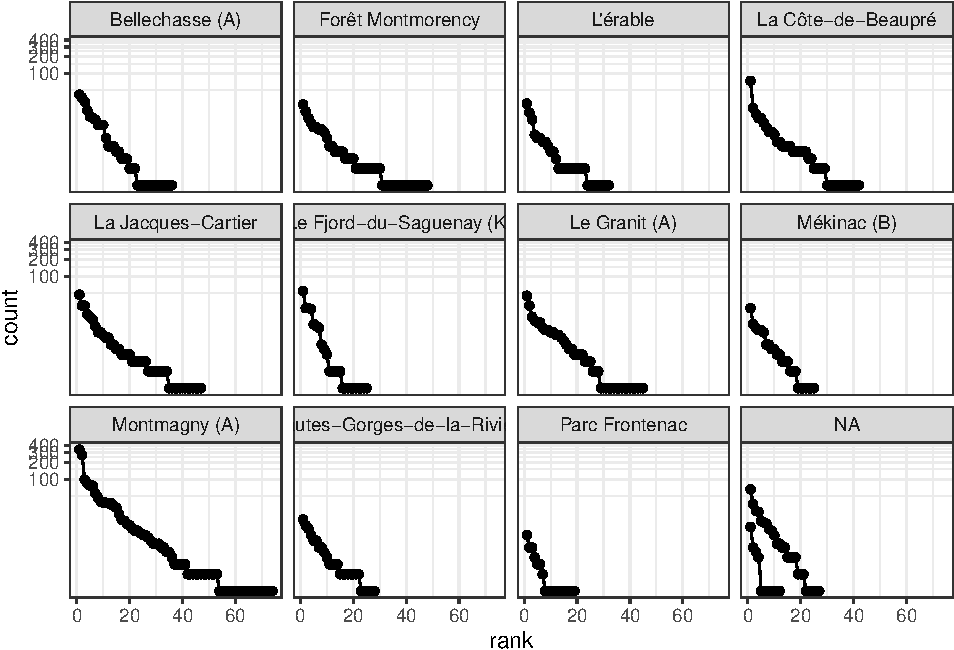
\includegraphics{indicators-bookdown_files/figure-latex/fig_rank_abd_insects_sol-1.pdf}

\hypertarget{questions-1}{%
\section{Questions}\label{questions-1}}

Why are some site names NA? do those sites not have names?

Should 0 values be uploaded into Coleo?

  \bibliography{book.bib,packages.bib}

\end{document}
